\usetikzlibrary{arrows.meta}

\begin{frame}[fragile,label=makeWhatRun]{exercise: what will run?}
\begin{tikzpicture}
\node[draw,very thick,align=left] (makefile) {
\tt
\begin{tabular}{l}
W: X Y \\
▶\hspace{1cm}buildW \\
X: Q \\
▶\hspace{1cm}buildX \\
Y: X Z \\
▶\hspace{1cm}buildY \\
\end{tabular}
};
\node[anchor=north west,align=left] at ([xshift=1cm]makefile.north east) {
\begin{tabular}{ll}
W & modified 1 minute ago \\
X & modified 3 hours ago \\
Y & does not exist \\
Z & modified 1 hour ago \\
Q & modified 2 hours ago \\
\end{tabular}
};
\end{tikzpicture}

exercise: ``make W'' will run what commands?
\vspace{.5cm}

\fontsize{13}{14}\selectfont
\begin{tabular}{lll}
A. none & B. \texttt{buildY} only & C. \texttt{buildW} then \texttt{buildY} \\
D. \texttt{buildY} then \texttt{buildW} & \multicolumn{2}{l}{E. \texttt{buildX} then \texttt{buildY} then \texttt{buildW}} \\
F. \texttt{buildX} then \texttt{buildW} & G. something else \\
\end{tabular}
\end{frame}

\begin{frame}<0>[fragile,label=makeWhatRunExplain]{explanation}
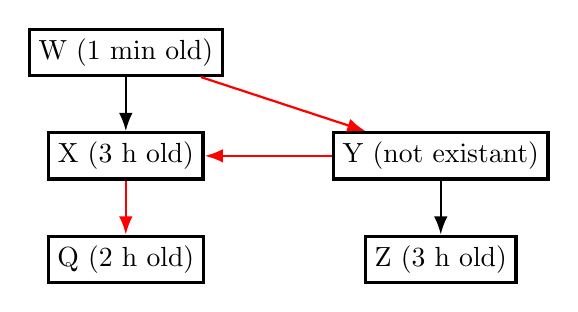
\begin{tikzpicture}
\begin{scope}[every node/.style={draw,very thick}]
\node (W) {W (1 min old)};
\node (X) at ([yshift=-1cm]W.south) {X (3 h old)};
\node (Y) at ([yshift=-1cm,xshift=4cm]W.south) {Y (not existant)};
\node (Q) at ([yshift=-1cm]X.south)  {Q (2 h old)};
\node (Z) at ([yshift=-1cm]Y.south)  {Z (3 h old)};
\end{scope}
\begin{scope}[-Latex,thick]
\draw (W) -- (X);
\draw[red] (W) -- (Y);
\draw[red] (X) -- (Q);
\draw[red] (Y) -- (X);
\draw (Y) -- (Z);
\end{scope}
\end{tikzpicture}
\end{frame}

\iftoggle{heldback}{}{\againframe<1->{makeWhatRunExplain}}
